% Preámbulo
\documentclass[stu, 12pt, letterpaper, donotrepeattitle, floatsintext, natbib]{apa7}
\usepackage[utf8]{inputenc}
\usepackage{comment}
\usepackage{marvosym}
\usepackage{graphicx}
\usepackage{float}
\usepackage[normalem]{ulem}
\usepackage[spanish]{babel} 
\usepackage{lastpage} %para le formato que quiere la profe QUITAR SI QUIERES OG APA7
\usepackage{ragged2e} %para le formato que quiere la profe QUITAR SI QUIERES OG APA7
\usepackage{indentfirst} %para le formato que quiere la profe QUITAR SI QUIERES OG APA7
\usepackage{multirow,booktabs,setspace,caption} %formato de figuras APA
\DeclareCaptionLabelSeparator*{spaced}{\\[2ex]}
\captionsetup[figure]{textfont=it,format=plain,justification=justified,
  singlelinecheck=false,labelsep=spaced,skip=0pt}

\selectlanguage{spanish}
\useunder{\uline}{\ul}{}
\newcommand{\myparagraph}[1]{\paragraph{#1}\mbox{}\\}

\rfoot{Página \thepage \hspace{1pt} de \pageref{LastPage}}%QUITAR SI QUIERES OG APA7 
\rhead{} %QUITAR SI QUIERES OG APA7
\setcounter{secnumdepth}{3} %permite enumerar las secciones QUITAR SI QUIERES OG APA7
\setlength{\parindent}{1.27cm} %sangria forzada QUITAR SI QUIERES OG APA7

% Portada
\thispagestyle{empty}
\title{\Large Hidrósfera, Litósfera y Atmósfera}
\author{Abraham Jhared Flores Azcona} % (autores separados, consultar al docente)
% Manera oficial de colocar los autores:
%\author{Autor(a) I, Autor(a) II, Autor(a) III, Autor(a) X}
\affiliation{Instituto Tecnológico de Tijuana}
\course{ACD-0908SC5C Desarrollo Sustentable}
\professor{M.C. Trinidad Castro Villa}
\duedate{22 de septiembre de 2021}

\renewcommand\labelitemi{$\bullet$}

\newcommand*\chem[1]{\ensuremath{\mathrm{#1}}}

\begin{document}
\maketitle


% Índices
\pagenumbering{arabic}
    % Contenido
\renewcommand\contentsname{Contenido}
\tableofcontents
\renewcommand{\listfigurename}{Figuras}
\listoffigures

% Cuerpo 
    %NOTA: PARA CITAR ESTILO "Merts (2003)" usar \cite{<nombre_cita_bib>}
    %                        "(Metz, 1978)" usar \citep{<nombre_cita_bib>}
\newpage
\section*{Introducción}
\addcontentsline{toc}{section}{Introducción}
Dentro \begin{justifying}
    de los conceptos de la hidrósfera, litósfera y atmósfera es comprensible el poder confundirse debido a los fonémas
    que se usan para escribirlos. Sus características de igual manera tienden a ser confusos por estar tan relacionados por lo que en esta breve
    redacción se sintetízan los conceptos y sus características para tener un mejor entendimiento de estas capas que conforman a la Tierra.\par
\end{justifying}
\section{Hidrósfera}
Se \begin{justifying}
    define como el componente de la Tierra el cual está compuesto de toda el agua líquida encontrable
    en el plantea. Se incluyen los oceanos, mares, lagos, estanques, rios y corrientas. Es el componente
    más grande de la Tierra; contando solamente a los oceanos, estos cubren alrededor del 71\% de la superficie
    terrestre. \citep{hanania-2016}
    \par
\end{justifying}
\begin{figure}[H]
    \caption{\emph{Ciclo del Agua}}
    \centering
    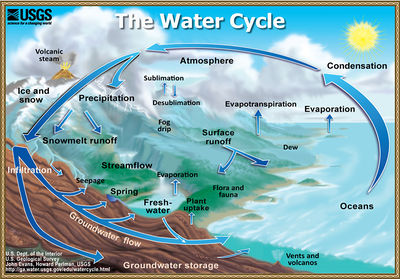
\includegraphics[width=14cm,height=10cm]{hydrosphere.jpg}
    \bigskip
    \\\small\textit{Nota}. La hidrósfera es el protagonista del ciclo. Tomado de \cite{hanania-2016}. %citar el de energyedu
\end{figure}
Es \begin{justifying}
    relevante destacar que a pesar de que la hidrósfera es compuesta principalmente por agua, existen algunos
    complementos que incluyen a los minerales, gases disueltos, y particulas de todo tipo; algunos de estos se pueden
    considerar contaminantes mientras que otros son vitales para la salud de los ecosistemas.\par
\end{justifying}
\vspace{\baselineskip}
\section{Litósfera}
Este \begin{justifying}
    forma el caparazón rigido de la Tierra. Esta incluye la corteza y, en cierta parte el manto superior llamado ``manto litosférico''. %citar al de cambridge
    La litósfera se diferencia de otras capas terrestres por la respuesta a los esfuerzos de deformación; esta
    es altamente viscosa y resistente a la deformación en los 100 km superiores del manto. \citep{penalba-2008}\par 
\end{justifying}
\begin{figure}[H]
    \caption{\emph{Capas de la Superficie Terrestre}}
    \centering
    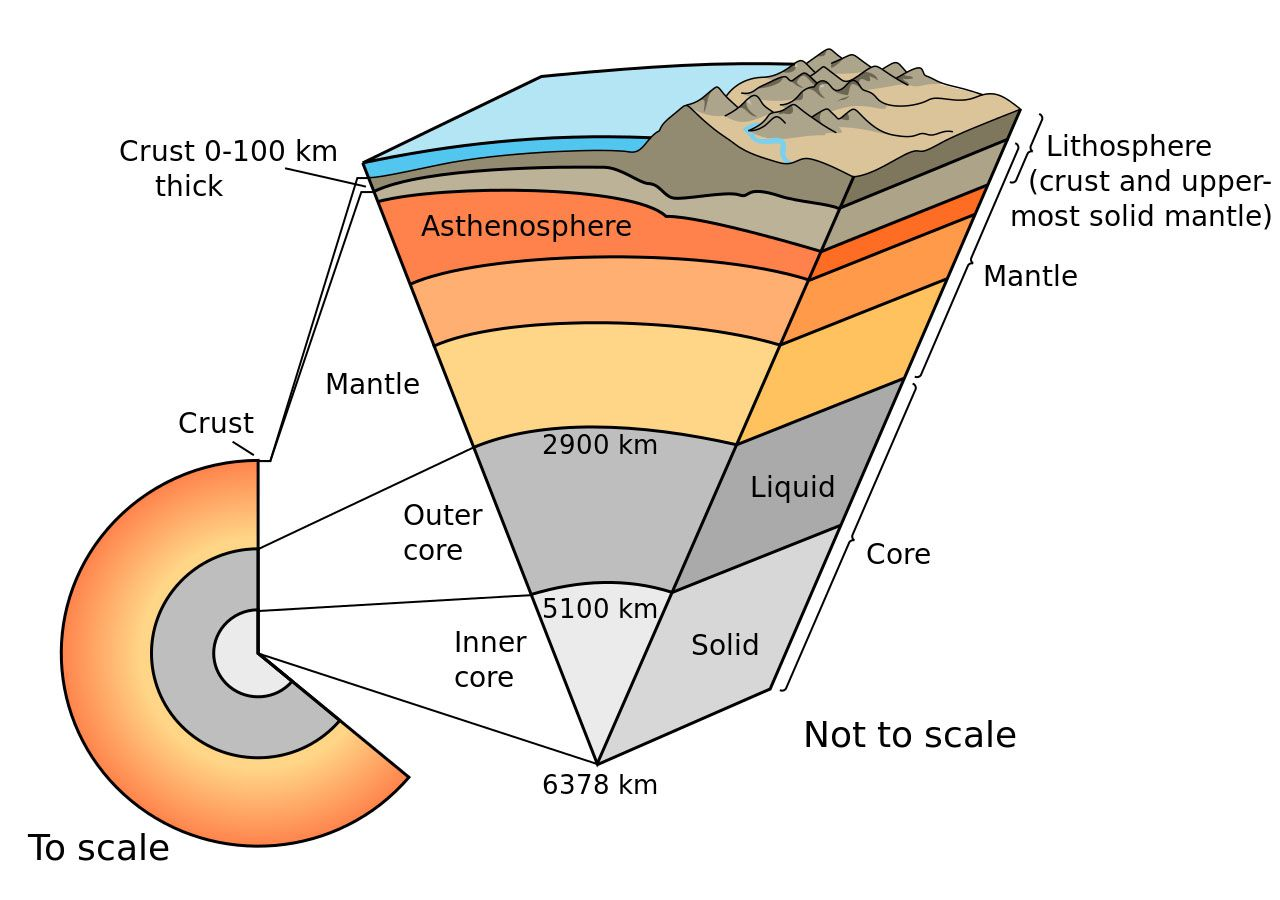
\includegraphics[width=14cm,height=10cm]{litosphere.jpg}
    \bigskip
    \\\small\textit{Nota}. La litósfera se encuentra en la parte superior. Tomado de \cite{unknown-author-no-dateA}. %citar el de natgeo
\end{figure}
\vspace{\baselineskip}
\section{Atmósfera}
A \begin{justifying}
    grandes rasgos, la atmósfera es una combinación de gases que rodea a la Tierra que permiten la posibilidad de vida en el planeta.
    Los gases predominantes en la atmósfera terrestre son el aire seco; compuesto de 78\% nitrógeno (\chem{N_2}) y alrededor de 21\% de oxígeno (\chem{O_2}).
    El resto de otros gases se presenta en menos del 1\% de la combinación de gases. \citep{unknown-author-no-dateB}\par %citar al de ucar
\end{justifying}
\vspace{\baselineskip}
\begin{figure}[H]
    \caption{\emph{Capas de la Atmósphera}}
    \centering
    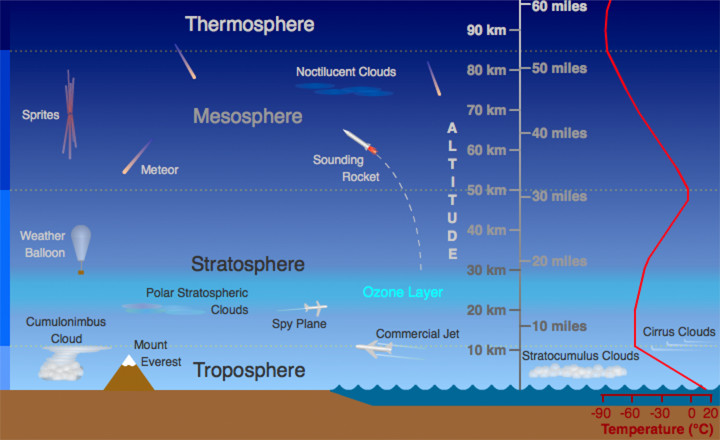
\includegraphics[width=14cm,height=10cm]{atmosphere.jpg}
    \bigskip
    \\\small\textit{Nota}. La vida se desarrolla en la tropósfera (troposphere). Tomado de \cite{russell-no-date}. %citar el otro de ucar
\end{figure}
\section*{Conclusión}
\addcontentsline{toc}{section}{Conclusión}
Para \begin{justifying}
    lo competente a la materia. Estudiar estas capas de la Tierra nos permiten comprender de una manera más elaborada los mecanismos los cuales
    conforman a la Tierra y por ende, la naturaleza para preveer posibles catástrofes naturales relacionadas a estas capas terrestres.\par
\end{justifying}

\newpage
% Referencias
\setcounter{secnumdepth}{0} %permite enumerar las secciones QUITAR SI QUIERES OG APA7
\renewcommand\refname{\textbf{Referencias}}
\bibliography{referencias}

\end{document}